
% this file is called up by thesis.tex
% content in this file will be fed into the main document
%: ----------------------- introduction file header -----------------------
\chapter{Introduction}

% the code below specifies where the figures are stored
\ifpdf
    \graphicspath{{1_introduction/figures/PNG/}{1_introduction/figures/PDF/}{1_introduction/figures/}}
\else
    \graphicspath{{1_introduction/figures/EPS/}{1_introduction/figures/}}
\fi

% ----------------------------------------------------------------------
%: ----------------------- introduction content ----------------------- 
% ----------------------------------------------------------------------



%: ----------------------- HELP: latex document organisation
% the commands below help you to subdivide and organise your thesis
%    \chapter{}       = level 1, top level
%    \section{}       = level 2
%    \subsection{}    = level 3
%    \subsubsection{} = level 4
% note that everything after the percentage sign is hidden from output



\section{Context} 
The LOw Frequency Array(LOFAR) telescope\footnote{\url{http://www.lofar.org/}} demands for huge data processing ability. 
It consists of 51 stations cross Europe and a typical LOFAR observation has the size of 100TB, after frequency averaging, the size can be reduced to 16TB. \cite{Spreeuw2019}
Collectively, there are over 5 PB of data will be stored each year. \cite{Start2020} In the data processing pipeline, the image calibration is a vital step. 
As the data collecting speed exceeds the capability of processing, the data will be stored and archived first. It will be feed to processing pipeline when it is needed.
The Netherlands eScience Center has developed solutions for calibrating imaged observation collected by LOFAR. The one of the way is sky map based direction independent calibration.
To calibrate the observation by given sky map, SAGECaL is invented and implemented for this purpose.\cite{Kazemi2011}. 
By given pre-processed observation data, sky model and parameters, the calibration can be done independently. 
However, it is a computation consuming application. Currently, eScience Center has developed GPU, MPI and Spark versions for acceleration.
All of them have achieved great acceleration compared to the naive uni-node version. 

However, under the huge requirement of computation, all three solutions have limitation. The GPU version provide no doubly great acceleration, which is in a sense vertical scaling.
MPI and Spark can be considered as horizontal scaling, GPU can provide support as well. But as it is said, LOAFR is cloud user and cloud provider in the same time, the resource utilization of their infrastructure is also important.
The MIP and Spark solutions may lead to waste of resources. The Fig. \ref{fig:sparkUti} gives an example that when the required computation resources decrease, idle resources(compute nodes) wouldn't be released by Spark.
On the other hand, a pure batch job system may enter a very special situation that a big job is waiting for resource while idle resources can not fulfill the requirement, for instance as shown in Fig. \ref{fig:MPIUti}.


% \begin{figure}
%     \centering
%     \begin{minipage}
%         \figuremacroW{1_introduction/figures/spark_NP.jpg}{Spark}{Spark occupys fixed resources}{0.45}
%     \end{minipage}
%     \begin{minipage}
%         \figuremacroW{1_introduction/figures/spark_NP.jpg}{Spark}{Spark occupys fixed resources}{0.45}
%     \end{minipage}
% \end{figure}

\begin{figure}
    \centering
    \begin{minipage}{.5\textwidth}
      \centering
      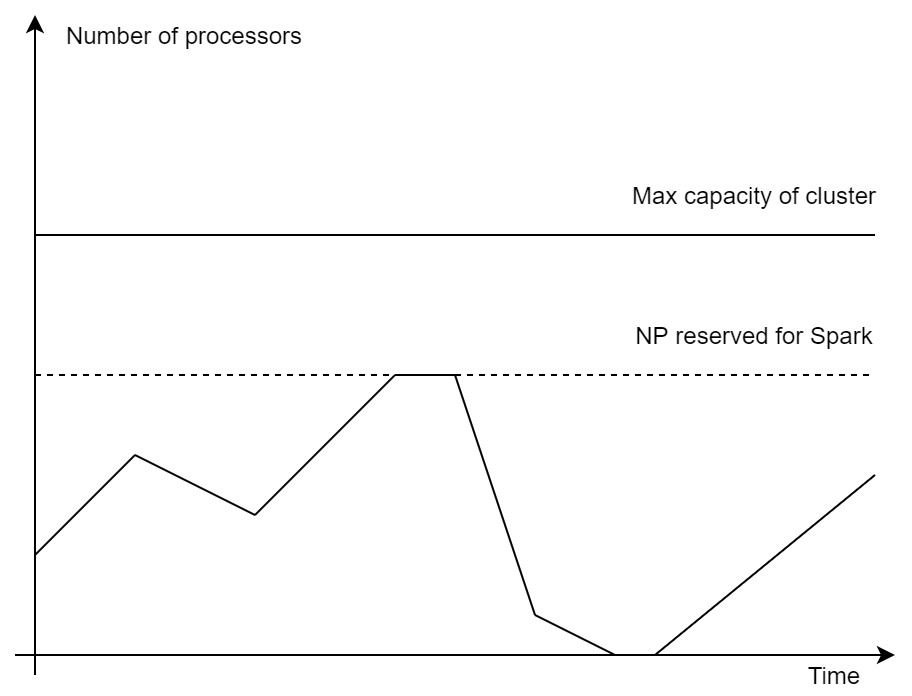
\includegraphics[width=0.9\linewidth]{1_introduction/figures/spark_NP.jpg}
      \caption[SparkUti]{{\small\textbf{Resource utilization by Spark} - Spark occupys fixed resources}}
      \label{fig:sparkUti}
    \end{minipage}%
    \begin{minipage}{.5\textwidth}
      \centering
      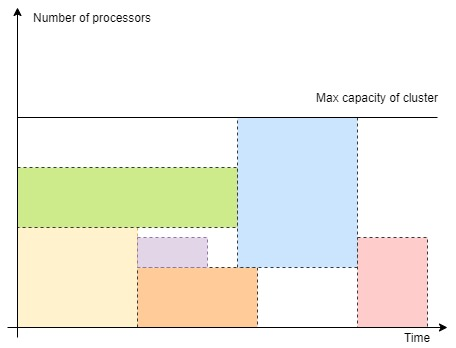
\includegraphics[width=0.9\linewidth]{1_introduction/figures/MPI_batch.jpg}
      \caption[MPIUti]{{\small\textbf{Resource utilization by MPI} - Too large jobs make resource waste}}
      \label{fig:MPIUti}
    \end{minipage}
\end{figure}
% \figuremacroW{1_introduction/figures/spark_NP.jpg}{Spark}{Spark occupys fixed resources}{0.45}
% \figuremacroW{1_introduction/figures/spark_NP.jpg}{Spark}{Spark occupys fixed resources}{0.45}
% \begin{figure}[htbp]
%     \centering
%     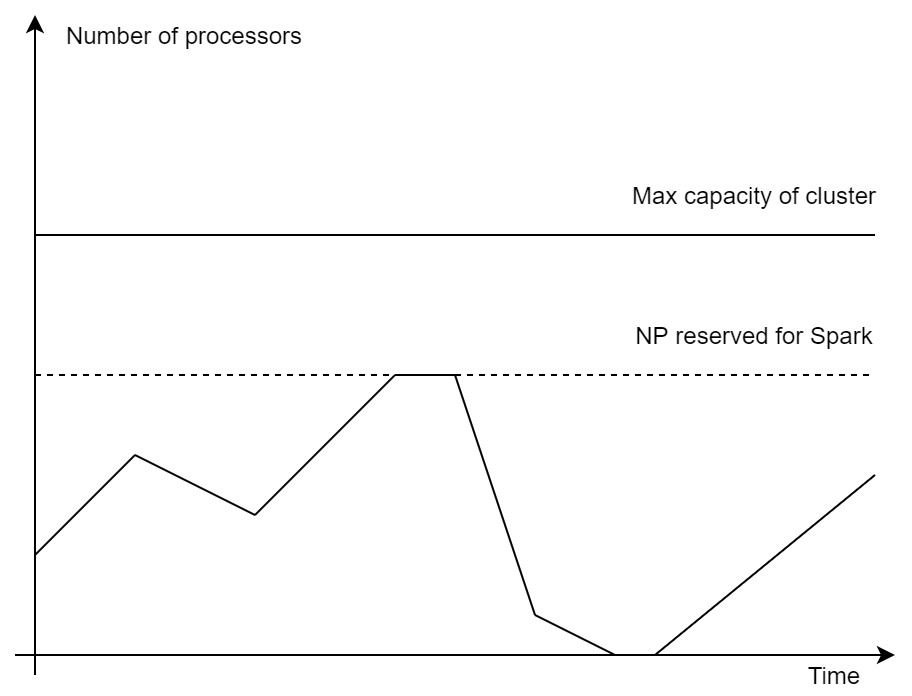
\includegraphics[width=\textwidth]{1_introduction/figures/spark_NP.jpg}
%     \caption[123]{123}
%     \label{134}
% \end{figure}

\section{Objective}

In the previous section, it is mentioned that LOAFR team has the role of both sides. Therefore, in this research, higher resource utilization of cloud system is the first objective.
In the same time, the acceleration of calibration processing is the second goal to achieve. Hopefully, the higher resource utilization, or in other words more active computation resources, is able to shrink the time for computing.

\section{Research Question}
The research question overall is how to implement an elastic distributed algorithm that can be auto-scaled dynamically that reduces the waste of resources.
More particularly, it can be extended into more specific questions:
\begin{itemize}
  \item How to set up an auto provisioning system adopting to the workload of a cloud that requests and releases resources dynamically?
  \item How to transform the calibration application into distributed and parallel version?
  \item How to make the distributed application capable to the dynamic scaling environment?
\end{itemize}


\section{Research Method}
The research method is practice based implementation plus comparison. 
In this research, firstly the previous work and current solutions will be explored. The limit, pros and cons of previous work will be collected and analyzed.
Secondly, a system that fulfills the demand of auto provisioning and overall higher resource utilization will be implemented.
Last, the system will be tested by given benchmark, and compared to other systems on the objective goals.

 
